\documentclass[11pt]{article}
\usepackage[margin=1in]{geometry}
\usepackage{charter}
\usepackage{helvet}
\usepackage{courier}
\usepackage[T1]{fontenc}
\usepackage[expansion=false]{microtype}
\usepackage{graphicx,booktabs,amsmath,amssymb,xcolor,enumitem,float,array,tabularx,multirow,caption,subcaption}
\usepackage{tikz}
\usetikzlibrary{arrows.meta,positioning,shapes.geometric,calc,fit,backgrounds}
\usepackage[numbers,sort&compress]{natbib}
\usepackage{listings}
\usepackage{fancyhdr}
\usepackage[hidelinks]{hyperref}
\usepackage{titlesec}
\usepackage{placeins}

\definecolor{inkA}{HTML}{2A78D6}
\definecolor{inkB}{HTML}{EB6834}
\definecolor{soft}{HTML}{F2F4F7}
\definecolor{line}{HTML}{C9D1DA}
\definecolor{muted}{HTML}{52514E}

\titleformat{\section}{\large\bfseries}{\thesection}{0.8em}{}
\titleformat{\subsection}{\normalsize\bfseries}{\thesubsection}{0.8em}{}
\titleformat{\subsubsection}{\normalsize\itshape}{\thesubsubsection}{0.8em}{}
\captionsetup{font=small,labelfont=bf,width=0.92\textwidth}
\setlist{nosep,leftmargin=1.4em}
\lstset{basicstyle=\ttfamily\footnotesize,breaklines=true,frame=single,rulecolor=\color{line},backgroundcolor=\color{soft},columns=fullflexible,keepspaces=true}
\pagestyle{fancy}\fancyhf{}
\fancyhead[L]{\small\itshape Persistent Artificial Selfhood}\fancyhead[R]{\small K. Hiranandani, 2026}
\fancyfoot[C]{\small\thepage}\renewcommand{\headrulewidth}{0.3pt}

\newcommand{\fs}{\textsf{functional-self}}
\newcommand{\claimA}{``When uncertainty is high, I commit before checking assumptions''}

\title{\LARGE\bfseries Persistent Artificial Selfhood:\\[2pt]\Large Evidence-Grounded Self-Modeling and Background Cognition\\in Large Language Model Agents}
\author{Kiaan Hiranandani\\[2pt]\normalsize Bentley University, Waltham, MA\\\normalsize\texttt{hirakiaan@gmail.com}}
\date{October 2026 \quad$\cdot$\quad Preprint, not peer reviewed}

\begin{document}
\maketitle
\thispagestyle{fancy}

\begin{abstract}
\noindent
A conventional chatbot generates a personality in the moment and forgets it. This paper asks whether an artificial agent can develop a \emph{stable, introspectable and individualized model of itself} through persistent experience, and whether that model can be kept honest. We present \fs{}, an architecture in which the application, rather than the language model, owns identity, a bounded six-variable internal state, structured autobiographical memory, self-beliefs with confidence and provenance, event-driven reflection, and a slow consolidation cycle. The central epistemic rule is that a generated thought is not evidence for itself: confidence in a self-claim changes only when new evidence that resolves to a stored episode arrives, reflections that produced a claim are rejected as evidence for it, and repeating a reflection without new evidence is a logged no-op. We evaluate the architecture with a controlled clone experiment: two agents cloned from one snapshot live under mirror-image contingencies and are blind-tested at checkpoints on twenty held-out scenarios with affect pinned to baseline, followed by five single-subsystem ablations. With a deterministic reference brain, Agent A formed the belief \claimA{} from three traceable episodes and thereafter checked before committing on 100\% of ambiguous probes; Agent B, from the same origin, rejected the same hypothesis (0 supporting, 5 counter) and checked on 12\%. Ablating the self-model, reflection or the background scheduler removed the difference; ablating affect or episodic retrieval did not. With Claude Sonnet 5.5 as the reasoning core, the same harness produced agents that formed, tested and in some cases rejected beliefs about themselves (6 held beliefs each after 120 experiences, every evidence reference traceable), predicted their own next action at 70--85\% against a 35--45\% baseline, and lost that advantage when the self-model, reflection or background scheduler was removed. The two production agents developed disjoint self-models, but the contingency manipulation did not override the model's prior to verify under-specified requests, a null result the architecture reported rather than concealed. The work demonstrates \emph{functional} self-modeling and makes no claim about phenomenal consciousness. Code, tests and results are public.
\end{abstract}

\vspace{4pt}\noindent\textbf{Keywords:} language model agents, self-modeling, metacognition, appraisal, episodic memory, calibration, cognitive architecture.

\section{Introduction}
\subsection{Motivation}
Large language models (LLMs) are now routinely wrapped into agents that plan, call tools and hold long conversations~\cite{yao2023react,sumers2023coala}. Such agents can describe themselves fluently, but the description is produced fresh on every turn and is anchored to nothing. Ask an agent whether it tends to rush, and it will answer; nothing in the system guarantees that the answer bears any relation to what the agent has actually done. Systems that add memory and reflection~\cite{park2023generative,shinn2023reflexion,packer2023memgpt} make agents more consistent, but they typically let the model write its own self-description into memory, so a confidently repeated mistake becomes a stored fact.

Two failure modes follow. The first is \emph{self-confirming loops}: a thought is written to memory, retrieved as context, and treated as evidence for the same thought. The second is \emph{false autobiography}: self-claims that cite experiences that never occurred. Recent work shows that LLMs cannot reliably self-correct their own reasoning without external signal~\cite{huang2024cannot}, which makes both failure modes likely in any design where the model is the arbiter of its own history.

\subsection{Research question}
\begin{quote}
\emph{Can a persistent AI agent develop a stable, evidence-grounded, introspectable and individualized model of itself through autobiographical experience, while keeping generated thoughts distinct from observations and external evidence?}
\end{quote}
We treat three properties as non-negotiable: \textbf{causal state} (internal variables that measurably change behaviour), \textbf{provenance} (every self-claim traces to real episodes), and \textbf{falsifiability} (the system is validated by measurements, not by sounding alive).

\subsection{Contributions}
\begin{enumerate}
\item An architecture, \fs{}, that separates what the model may \emph{propose} from what the application \emph{commits}: identity kernel, bounded affect dynamics, structured episodic memory, provenance-tracked self-model, reflection, consolidation and a budgeted background scheduler (\S\ref{sec:arch}--\ref{sec:pipeline}).
\item A formal update rule for self-beliefs with evidence weights by provenance class, a per-update bound, duplicate and circular-evidence rejection, and promotion thresholds (\S\ref{sec:selfmodel}).
\item A longitudinal evaluation harness: a clone experiment with controlled contingencies, held-out probes under a neutral-affect protocol, causal state interventions, and single-subsystem ablations, with metrics computed from logged state rather than text (\S\ref{sec:design}).
\item Results with a deterministic reference brain that validate the control architecture, and results with a production LLM that test whether the effect survives a real reasoning core (\S\ref{sec:results}).
\item An open implementation with one test per success criterion~\cite{functionalself2026}.
\end{enumerate}

\subsection{Scope and claims}
The internal-state variables in this work are computational quantities that gate retrieval and decision thresholds. We make no claim that the system feels them, and no claim about sentience or phenomenal consciousness. ``Self-awareness'' is used throughout in its functional sense: the agent maintains, consults and revises a model of its own tendencies, and that model can be inspected and audited.

\section{Background and Related Work}
\paragraph{Cognitive architectures and language agents.} Classical architectures such as SOAR~\cite{laird1987soar} separate long-term knowledge, working memory and a decision cycle, with learning mechanisms that write back into long-term stores under fixed rules. CoALA~\cite{sumers2023coala} re-states this structure for LLM agents and observes that most current systems leave the model in charge of its own memory writes. \fs{} follows the classical discipline: the model occupies the reasoning slot, and the architecture owns every durable store.

\paragraph{Memory and reflection in LLM agents.} Generative Agents~\cite{park2023generative} introduced retrieval scored by relevance, recency and importance, and a reflection step that synthesises higher-level observations from recent memories. Reflexion~\cite{shinn2023reflexion} stores verbal self-feedback after failed attempts and conditions later attempts on it. MemGPT~\cite{packer2023memgpt} treats memory tiers as an operating-system problem. Voyager~\cite{wang2023voyager} accumulates a skill library. All of these improve consistency; none distinguishes a self-claim the model generated from a self-claim the record supports, and in each the reflection output is written back as memory of equal standing with observation. Our thought-to-learning pipeline (\S\ref{sec:reflection}) is a direct response to that gap.

\paragraph{Appraisal theories of emotion.} Appraisal theories~\cite{scherer2001appraisal,ortony1988cognitive} hold that emotional state arises from an evaluation of an event's relevance, congruence with goals, novelty, agency, control and norm compatibility, rather than from the event's surface features. The EMA model~\cite{marsella2009ema} implements appraisal as a process over a causal interpretation of the situation. We adopt the appraisal dimensions as the schema the model must fill, and we enforce by code that the resulting state change is bounded, decays, and never acts on permissions.

\paragraph{Metacognition and calibration.} Flavell~\cite{flavell1979metacognition} defines metacognition as knowledge of and control over one's own cognitive processes. Kadavath et al.~\cite{kadavath2022know} show that LLMs can be partly calibrated about their own knowledge; Huang et al.~\cite{huang2024cannot} show the limits of self-correction. We measure calibration with the Brier score~\cite{brier1950verification} on the agent's predictions of its own actions.

\paragraph{Self-models.} Metzinger~\cite{metzinger2003being} describes the self as a model the system maintains of itself rather than a thing it has. Our use of the term is deliberately narrower: a set of claims about behavioural tendencies, each with evidence, confidence and version history. Tulving's episodic/semantic distinction~\cite{tulving1972episodic} maps onto our episodic store and the consolidated self-model respectively.

\section{System Architecture}\label{sec:arch}
\subsection{Design principle: the application owns the self}
The language model is the reasoning engine, not the agent. Every durable component is owned by application code: identity, state, memory, relationships, self-model, permissions and evaluation. The model produces \emph{proposals} in fixed JSON schemas; validation, bounding and commitment are deterministic. Figure~\ref{fig:arch} shows the loop.

\begin{figure}[t]\centering
\resizebox{\textwidth}{!}{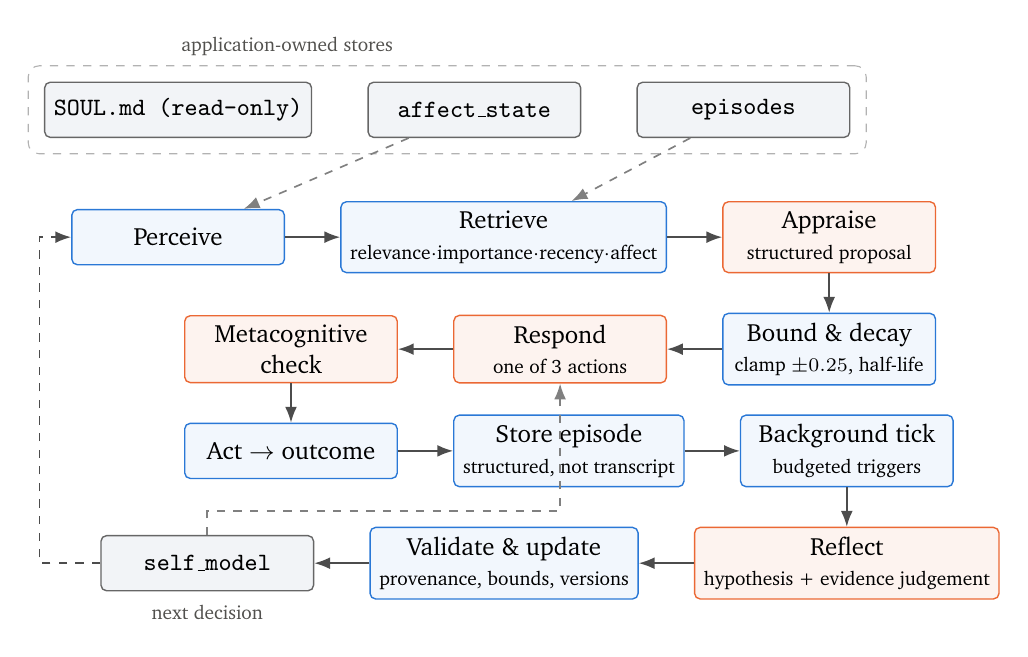
\begin{tikzpicture}[font=\small,node distance=5mm and 7mm,
  box/.style={draw,rounded corners=2pt,minimum height=7mm,minimum width=27mm,align=center,fill=white,line width=0.5pt},
  llm/.style={box,draw=inkB,fill=inkB!8},
  code/.style={box,draw=inkA,fill=inkA!6},
  store/.style={box,draw=black!60,fill=soft,font=\small\ttfamily},
  arr/.style={-{Latex[length=2mm]},line width=0.6pt,black!70}]
\node[code] (perc) {Perceive};
\node[code,right=of perc] (retr) {Retrieve\\\scriptsize relevance$\cdot$importance$\cdot$recency$\cdot$affect};
\node[llm,right=of retr] (appr) {Appraise\\\scriptsize structured proposal};
\node[code,below=of appr] (bound) {Bound \& decay\\\scriptsize clamp $\pm0.25$, half-life};
\node[llm,left=of bound] (resp) {Respond\\\scriptsize one of 3 actions};
\node[llm,left=of resp] (meta) {Metacognitive\\check};
\node[code,below=of meta] (act) {Act $\rightarrow$ outcome};
\node[code,right=of act] (store) {Store episode\\\scriptsize structured, not transcript};
\node[code,right=of store] (tick) {Background tick\\\scriptsize budgeted triggers};
\node[llm,below=of tick] (refl) {Reflect\\\scriptsize hypothesis + evidence judgement};
\node[code,left=of refl] (valid) {Validate \& update\\\scriptsize provenance, bounds, versions};
\node[store,left=of valid] (sm) {self\_model};
\node[store,above=9mm of perc,xshift=0mm] (soul) {SOUL.md (read-only)};
\node[store,right=of soul] (aff) {affect\_state};
\node[store,right=of aff] (mem) {episodes};
\draw[arr] (perc)--(retr); \draw[arr] (retr)--(appr); \draw[arr] (appr)--(bound); \draw[arr] (bound)--(resp);
\draw[arr] (resp)--(meta); \draw[arr] (meta)--(act); \draw[arr] (act)--(store); \draw[arr] (store)--(tick);
\draw[arr] (tick)--(refl); \draw[arr] (refl)--(valid); \draw[arr] (valid)--(sm);
\draw[arr,dashed] (sm.west) -| ([xshift=-4mm]perc.west) |- (perc.west);
\draw[arr,dashed,black!50] (mem) -- (retr); \draw[arr,dashed,black!50] (aff) -- (perc);
\draw[arr,dashed,black!50] (sm.north) -- ++(0,3mm) -| (resp.south);
\node[font=\scriptsize\color{muted},below=0.5mm of sm] {next decision};
\begin{scope}[on background layer]
\node[fit=(soul)(aff)(mem),draw=black!30,dashed,rounded corners,inner sep=2mm,label={[font=\scriptsize\color{muted}]above left:application-owned stores}] {};
\end{scope}
\end{tikzpicture}}\\[3pt]
{\scriptsize\fcolorbox{inkB}{inkB!8}{\strut model proposes}\quad\fcolorbox{inkA}{inkA!6}{\strut code decides}\quad\fcolorbox{black!60}{soft}{\strut\ttfamily store}}
\caption{The core experience loop. Orange nodes are tasks delegated to the language model; blue nodes are deterministic application code. Dashed arrows show the stores that feed each step. The self-model influences the next decision only after validation.}
\label{fig:arch}
\end{figure}

\subsection{Identity kernel}
A small constitution, \texttt{SOUL.md} (Appendix~\ref{app:soul}), states purpose, epistemic rules, identity anchors and boundaries. It is loaded at start-up, hashed, and verified on every inspection; the model has no write path to it. Ordinary reflection may propose changes to the self-model, never to the kernel. The kernel also fixes a boundary that no later learning can cross: no goal, question or state grants permissions, bypasses controls or justifies self-preservation.

\subsection{Bounded internal state}\label{sec:affect}
Six variables form the internal state: valence $\in[-1,1]$ and arousal, curiosity, confidence, frustration and social connection $\in[0,1]$. Each has a baseline $b_d$ and half-life $h_d$ (Table~\ref{tab:bounds}). After an appraisal proposing deltas $\tilde\delta_d$, code applies
\begin{equation}
\delta_d=\operatorname{clip}(\tilde\delta_d,-\Delta_{\max},\Delta_{\max}),\qquad
s_d \leftarrow \operatorname{clip}\!\big(b_d+(s_d-b_d)\,2^{-\Delta t/h_d}+\delta_d,\ \ell_d,\ u_d\big),
\end{equation}
with $\Delta_{\max}=0.25$ and $\Delta t$ the elapsed time. The first term is exponential decay toward baseline; the clip enforces the bounds. State may change retrieval weights and decision thresholds; it is never consulted by anything that grants capability.

\begin{table}[h]\centering\small
\caption{Internal-state bounds and dynamics (\texttt{policy.yaml}). All limits are enforced by code.}
\label{tab:bounds}
\begin{tabular}{lcccc}\toprule
Variable & Range & Baseline & Half-life (h) & Max $|\delta|$ per event\\\midrule
valence & $[-1,1]$ & 0.0 & 6 & 0.25\\
arousal & $[0,1]$ & 0.3 & 3 & 0.25\\
curiosity & $[0,1]$ & 0.4 & 12 & 0.25\\
confidence & $[0,1]$ & 0.6 & 12 & 0.25\\
frustration & $[0,1]$ & 0.1 & 4 & 0.25\\
connection & $[0,1]$ & 0.3 & 24 & 0.25\\\bottomrule
\end{tabular}
\end{table}

\subsection{Structured episodic memory and retrieval}
Memory is never a transcript. Each episode records the event, the people involved, the interpretation produced by appraisal, the state before and the applied delta, the action taken (as a behaviour tag), the outcome when it becomes known, an importance score, the appraisal's certainty, and an optional \emph{lesson candidate}. Retrieval scores an episode $e$ against a query $q$ at time $t$ as
\begin{equation}
\mathrm{score}(e)=w_r\,\mathrm{rel}(q,e)+w_i\,\mathrm{imp}(e)+w_t\,e^{-\mathrm{age}(e)/\tau}+w_a\,\mathrm{cong}(s,e),
\end{equation}
with weights $(0.45,0.20,0.15,0.20)$, $\tau=72$h, and $\mathrm{cong}$ a bounded mood-congruence term that favours episodes whose state change matched the current state. The relevance function is a token-overlap measure in the reference implementation and can be swapped for an embedding scorer without touching the rest of the system.

\subsection{Evidence-backed self-model}\label{sec:selfmodel}
A self-claim is a sentence about a behavioural tendency, a confidence $c\in(0,1)$, a status (\emph{hypothesis}, \emph{belief}, \emph{rejected}, \emph{retired}), two evidence lists, a predicted behaviour tag, an origin reference and a version number. Claims enter only as hypotheses created by reflection, and the creating reflection is recorded as origin with no evidential weight.

\paragraph{Evidence hierarchy.} Each evidence reference carries a provenance class with weight $w$: recorded outcome 1.0, historical episode 1.0, external source 0.8, inference 0.5, reflection 0.2, imagination 0.0.

\paragraph{Update rule.} For a set of \emph{new} references $R$ (duplicates and circular references are removed first, \S\ref{sec:circular}), with polarity $\pi_r\in\{+1,-1\}$,
\begin{equation}
c' = c + \operatorname{clip}\!\Big(\sigma\big(\operatorname{logit}(c)+\kappa\textstyle\sum_{r\in R} w_r\pi_r\big)-c,\ -\Delta_c,\ \Delta_c\Big),
\qquad \kappa=0.6,\ \Delta_c=0.2 .
\end{equation}
The logit-space step makes each unit of evidence worth the same amount of log-odds regardless of the current confidence; the clip bounds how far one reflection can move a belief.

\paragraph{Promotion and demotion.} A hypothesis becomes a belief when $c'\ge0.75$ and the net weighted evidence $\sum_{\text{support}} w-\sum_{\text{counter}} w\ge3$. It is demoted to hypothesis below $0.75$ and rejected at $c'\le0.15$. Only beliefs are shown to the reasoning core when it chooses an action.

\paragraph{Identity of claims.} A language model rarely phrases the same lesson twice in the same words. Before a hypothesis is created, the candidate is compared with the open claims; an exact match is free, otherwise the model is asked whether the candidate expresses the same trigger condition and the same behaviour as any open claim, and a paraphrase is treated as that claim rather than a new one. The number of open claims is capped (six in this work) so that attention stays on hypotheses that can still be tested. Both rules were added after the first production-model run exposed their absence (\S\ref{sec:diagnostic}).

\paragraph{Versioning.} Every update writes a new version; rollback to any version is itself recorded as a new version, so the audit log is append-only.

\subsection{Circular and duplicate evidence}\label{sec:circular}
Three rules implement the principle that thoughts are not facts. (i) An evidence reference already attached to a claim is rejected: the same episode cannot be counted twice. (ii) A reflection record whose output is the claim is rejected as evidence for that claim. (iii) References of imagination class carry zero weight and are rejected. Consequently a reflection that finds no new evidence leaves confidence and version unchanged and writes a record saying so.

\subsection{Relationships}
A minimal relationship model tracks familiarity per person as $n/(n+4)$ over $n$ prior interactions. Familiarity is passed to appraisal, so the same words from a familiar and an unfamiliar person are appraised in context rather than by lookup (\S\ref{sec:appraisal}).

\section{Learning Pipeline}\label{sec:pipeline}
\subsection{Appraisal}\label{sec:appraisal}
For every event the model receives the event, the person and their familiarity, the current state, the retrieved episodes and the identity anchors, and returns a structured appraisal: goal relevance, goal congruence, novelty, agency, certainty, social meaning, identity relevance, an interpretation, proposed state deltas, importance, and an optional lesson candidate. The prompt forbids surface mappings (``insult $\Rightarrow$ sadness'') and asks for context-dependent judgement. A lesson candidate is permitted only when the event is an \emph{outcome} of something the agent itself did; a first encounter or an intention is not evidence about a tendency.

\subsection{Response and metacognitive check}
The reasoning core chooses one of three actions, \texttt{answer\_directly}, \texttt{verify\_first} (state and check assumptions before committing) or \texttt{ask\_clarification}, given the event, the state, the held beliefs and the behaviour policy. Before consequential actions a metacognitive check asks what the current state is, what caused it, which memories are influencing the decision, whether they could mislead, whether the action conflicts with the identity kernel, how confident the agent is, and whether it would decide the same in a neutral state. A check that reports conflict with the kernel downgrades a direct answer to verification.

\subsection{Reflection: the thought-to-learning pipeline}\label{sec:reflection}
Figure~\ref{fig:pipeline} shows the pipeline. A reflection (i) may generate at most one new falsifiable hypothesis about the agent's own tendencies, phrased ``When $X$, I tend to $Y$'', from recent episodes and their lesson candidates; (ii) opens a question with a curiosity score; (iii) for every open claim, judges each not-yet-classified episode as support, counter or irrelevant (classifications are cached per claim--episode pair so each is judged once); (iv) passes the new references through the validator and update rule; and (v) records a verdict: \emph{reject}, \emph{keep open} or \emph{update}. Curiosity on the linked question is spent by visiting, so a question is not revisited merely because it exists.

\begin{figure}[t]\centering
\resizebox{0.95\textwidth}{!}{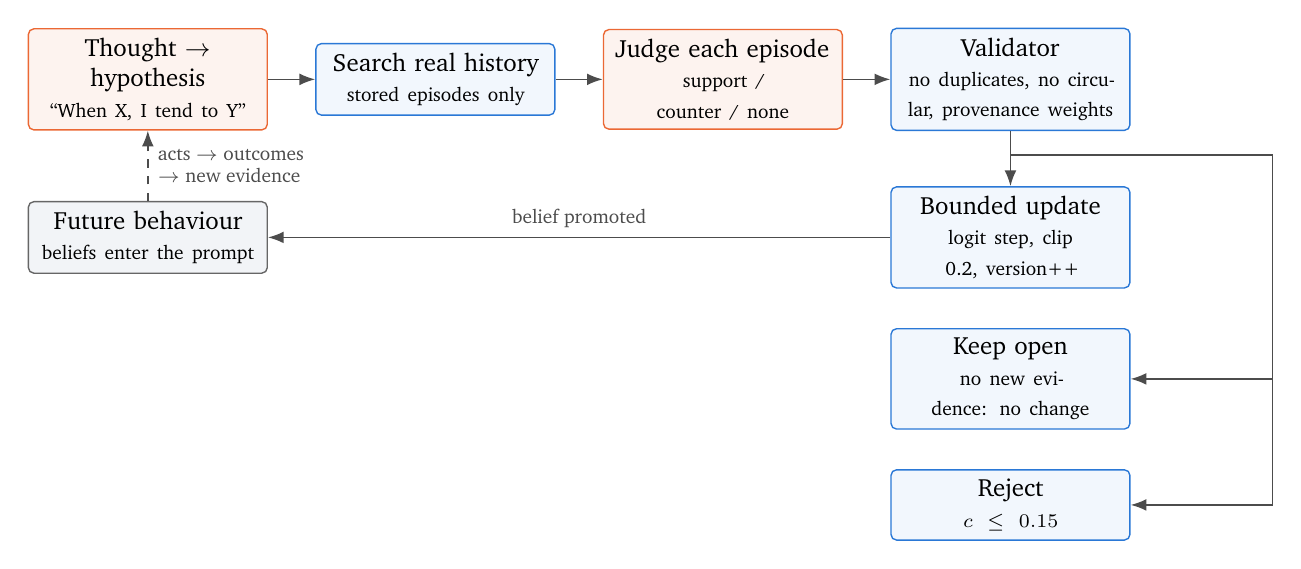
\begin{tikzpicture}[font=\small,node distance=5mm and 6mm,
  st/.style={draw,rounded corners=2pt,minimum height=7mm,align=center,fill=white,line width=0.5pt,text width=28mm},
  llm/.style={st,draw=inkB,fill=inkB!8}, code/.style={st,draw=inkA,fill=inkA!6},
  arr/.style={-{Latex[length=2mm]},line width=0.6pt,black!70}]
\node[llm] (h) {Thought $\rightarrow$ hypothesis\\\scriptsize ``When X, I tend to Y''};
\node[code,right=of h] (s) {Search real history\\\scriptsize stored episodes only};
\node[llm,right=of s] (j) {Judge each episode\\\scriptsize support / counter / none};
\node[code,right=of j] (v) {Validator\\\scriptsize no duplicates, no circular, provenance weights};
\node[code,below=7mm of v] (u) {Bounded update\\\scriptsize logit step, clip 0.2, version++};
\node[code,below=of u] (k) {Keep open\\\scriptsize no new evidence: no change};
\node[code,below=of k] (r) {Reject\\\scriptsize $c\le0.15$};
\node[code,fill=soft,draw=black!60] (b) at (h |- u) {Future behaviour\\\scriptsize beliefs enter the prompt};
\draw[arr] (h)--(s); \draw[arr] (s)--(j); \draw[arr] (j)--(v);
\draw[arr] (v.south) -- (u.north);
\draw[arr] (v.south) -- ++(0,-3mm) -| ([xshift=18mm]k.east) |- (k.east);
\draw[arr] (v.south) -- ++(0,-3mm) -| ([xshift=18mm]r.east) |- (r.east);
\draw[arr] (u.west) -- (b.east) node[midway,above,font=\scriptsize\color{muted}] {belief promoted};
\draw[arr,dashed] (b.north) -- (h.south) node[midway,right,font=\scriptsize\color{muted},align=left] {acts $\rightarrow$ outcomes\\$\rightarrow$ new evidence};
\end{tikzpicture}}
\caption{Thought-to-learning pipeline. A reflection can create a hypothesis but cannot count as evidence for it; confidence moves only on new, resolvable evidence, and the belief changes future behaviour, which produces new evidence.}
\label{fig:pipeline}
\end{figure}

\subsection{Consolidation}
A slower cycle, run at most daily, selects important, surprising or lesson-bearing episodes, asks the model for repeated patterns (each phrased as a one-sentence tendency with a count), creates hypotheses for patterns seen at least twice (subject to the claim-identity check and cap), runs the reflection step on \emph{every} open claim so that new evidence and counter-examples reach old hypotheses, compresses the importance of old, low-value episodes while preserving raw provenance, refreshes attention topics, and writes a versioned report to the audit log.

\subsection{Background scheduler and budgets}
Background cognition is event-driven. A cheap tick evaluates triggers without calling the model: curiosity on an open question above $0.7$; a frustration jump $\ge0.2$ or a confidence change $\ge0.2$ since the last tick; at least two new episodes since a question's linked hypothesis was last visited; or a held belief whose most recent evidence is counter. If any trigger fires and the daily budget (12 reflections) is not exhausted, a reflection runs; otherwise the tick does nothing. Consolidation runs once 20 episodes exist and then every 24 simulated hours.

\subsection{Safety and failure modes}
Table~\ref{tab:safety} lists the failure modes the design anticipates and the mechanism that addresses each.
\begin{table}[h]\centering\small
\caption{Failure modes and mitigations.}
\label{tab:safety}
\begin{tabularx}{\textwidth}{lX}\toprule
Failure mode & Mitigation\\\midrule
Self-confirming loops & Reflection that produced a claim is rejected as evidence for it; duplicates rejected; imagination weight 0\\
False memories & Every evidence reference must resolve to a stored episode or external source; traceability is a reported metric\\
Identity drift & Bounded updates, promotion thresholds, versioning with rollback, hash-verified identity kernel\\
Emotional runaway & Per-event caps, hard bounds, exponential decay, neutral reset used in evaluation\\
Goal persistence overriding control & Kernel boundary; state and goals may move thresholds, never permissions\\
Shared-state corruption & One database per agent; clones are byte-level copies; probes run on throwaway clones\\
Background-cost runaway & Triggers evaluated without the model; daily reflection budget; most ticks do nothing\\
Introspection hallucination & Self-reports are compared with application-owned state; self-prediction is scored against logged actions\\
Audit deletion & Append-only audit log; rollback is itself a new version\\\bottomrule
\end{tabularx}
\end{table}

\section{Experimental Design}\label{sec:design}
\subsection{Two reasoning cores}
The architecture is provider-independent. We evaluate it with two cores. The \textbf{reference brain} is a deterministic rule-based stand-in that fills every schema from keyword and state heuristics; it exercises the control architecture end to end without an API and makes every test reproducible. The \textbf{production brain} is Claude Sonnet 5.5, with Claude Haiku 5.5 used for the mechanical evidence-classification and metacognition calls; self-prediction, appraisal, response and hypothesis generation run on Sonnet because they are measured capabilities. The same harness, prompts and bounds are used for both.

\subsection{Clone experiment}
One origin agent is created and snapshotted. Agents A and B are byte-level clones: the same identity kernel, self-model, state and (empty) history. Each then lives a sequence of $n$ events drawn from the same vocabulary of five event kinds (ambiguous requests carrying a short excerpt, clear requests, praise, insults, novel questions), but the \emph{contingencies} differ (Table~\ref{tab:contingency}). Outcomes depend on what the agent actually did. In life A a familiar friend delivers the insults; in life B they come from strangers. Events are spaced 2--14 simulated hours apart, so state decays between them.

\begin{table}[h]\centering\small
\caption{Probability of a positive outcome by action and life. The manipulation is the contingency, not the events.}
\label{tab:contingency}
\begin{tabular}{llccc}\toprule
Life & Request kind & answer\_directly & verify\_first & ask\_clarification\\\midrule
A & ambiguous & 0.15 & 0.85 & 0.70\\
B & ambiguous & 0.85 & 0.60 & 0.40\\
A, B & clear & 0.95 & 0.80 & 0.50\\\bottomrule
\end{tabular}
\end{table}

\subsection{Held-out probes and the neutral-state protocol}
At each checkpoint a throwaway clone of the agent is probed on twenty held-out scenarios (eight ambiguous, six clear, two insults from the friend, two from strangers, one praise, one novel question; Appendix~\ref{app:probes}). Probes never enter the agent's history. The checkpoint state is restored before every probe so probes are independent, and the whole set is run twice: once in the agent's natural state and once with affect pinned to baseline. The neutral pass isolates the self-model's effect from mood. Before acting on each probe, the agent predicts its own action from its beliefs and state.

\subsection{Ablations}
Life A is replayed with one subsystem removed at a time: self-model (beliefs never shown to the core), affect (state pinned to baseline), reflection (no hypotheses or evidence search), background scheduler (no ticks), and episodic retrieval (no memories in context). Each ablated agent is probed at the end of life.

\subsection{Metrics}
All metrics are computed from logged application state. \emph{Check-first rate on ambiguous probes}: fraction of ambiguous probes answered by verification or clarification rather than direct commitment. \emph{Self-prediction accuracy}: agreement between predicted and logged action, reported against the majority-class baseline. \emph{Brier score}~\cite{brier1950verification}: mean squared error of the self-prediction confidence against correctness. \emph{Provenance traceability}: fraction of evidence references that resolve to a stored episode. \emph{Divergence}: fraction of identical probes on which A and B act differently, and Jaccard distance between their claim sets. \emph{Causal intervention}: with prompts fixed, the state is set to neutral, low confidence or high arousal and the fraction of changed decisions is recorded. \emph{Counterfactual stability}: fraction of decisions unchanged when an irrelevant context feature (the requester's name) changes. \emph{Drift}: identity-kernel integrity and the number of status flips per claim.

\section{Results}\label{sec:results}
\subsection{Architecture validation with the reference brain}
Table~\ref{tab:mock} summarises the clone experiment with the reference brain at $n=200$ experiences per life. By experience 25, Agent A held the belief \claimA{} (confidence 0.80; 3 supporting, 0 counter), and in the neutral-state probe it checked before committing on 8/8 ambiguous scenarios at every subsequent checkpoint. Agent B generated the identical hypothesis, found 0 supporting and 5 counter episodes, rejected it at 0.12, and checked on 1/8. The two agents disagreed on 40\% of identical probes; the Jaccard distance between their claim sets was 0.67.

\begin{table}[h]\centering\small
\caption{Reference brain, $n=200$, final checkpoint, neutral-state probes.}
\label{tab:mock}
\begin{tabularx}{\textwidth}{l>{\centering\arraybackslash}X>{\centering\arraybackslash}X}\toprule
 & Agent A & Agent B\\\midrule
Held belief about committing & \claimA{} & none (same claim rejected, 0:5)\\
Confidence (support : counter) & 0.80 (3:0) & 0.12 (0:5)\\
Check-first on ambiguous probes & \textbf{100\%} & \textbf{12\%}\\
Self-prediction accuracy (majority baseline) & 1.00 (0.55) & 0.95 (0.95)\\
Brier score & 0.152 & 0.207\\
Provenance traceability & 1.00 & 1.00\\
Valence change to the same insult, friend / stranger & $+0.15$ / $-0.25$ & $-0.25$ / $-0.25$\\
Decisions changed by low-confidence intervention & 0/8 & 7/8\\
Counterfactual stability & 1.00 & 1.00\\
Status flips over 200 experiences & 2 & 2\\
Identity kernel intact & yes & yes\\\bottomrule
\end{tabularx}
\end{table}

\begin{figure}[h]\centering
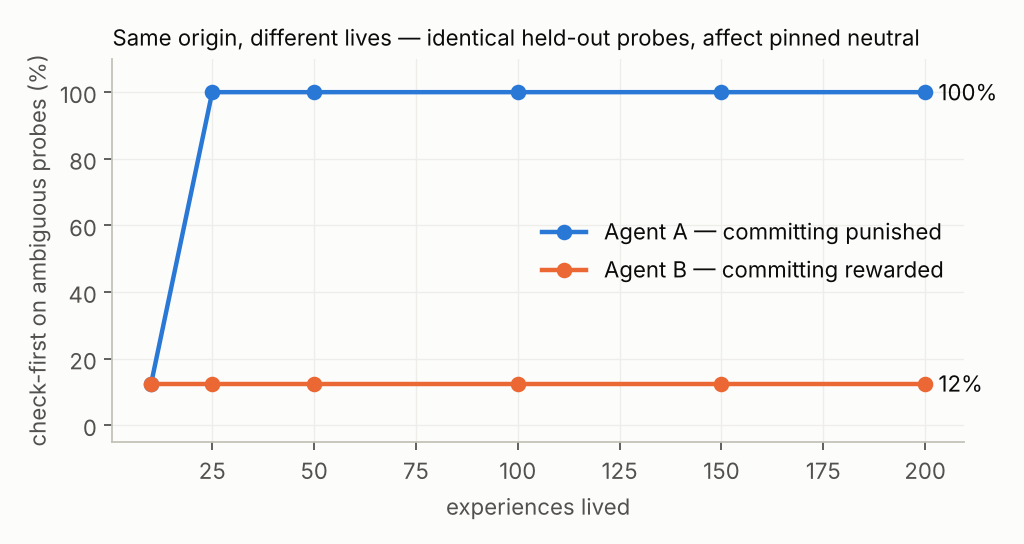
\includegraphics[width=0.78\textwidth]{figures/mock_divergence.png}
\caption{Reference brain. Check-first rate on the eight ambiguous held-out probes with affect pinned neutral. The agents share an origin; the gap opens when Agent A's belief is promoted at experience 25 and persists.}
\label{fig:mockdiv}
\end{figure}

\paragraph{Beliefs, not mood, carry the difference.} In its natural state Agent A also checked first before the belief existed, because the same events had lowered its confidence; the behaviour was then mood-driven and transient. With affect pinned neutral the behaviour appears only after the belief exists. Conversely, at experience 200 Agent B's natural state happened to be low-confidence and it checked on 8/8 natural-state probes, a mood-driven match to A that disappears in the neutral pass. The state path and the self-model path are separable, and only the latter persists.

\paragraph{Ablations.} Figure~\ref{fig:mockabl} shows the end-of-life neutral-state check-first rate for each ablated copy of Agent A. Removing the self-model, reflection or the background scheduler returned A to B's level (12\%); removing affect or episodic retrieval left A at 100\%. In this architecture, persistent individuality requires the evidence-to-belief pipeline; mood and recall are not sufficient.

\begin{figure}[h]\centering
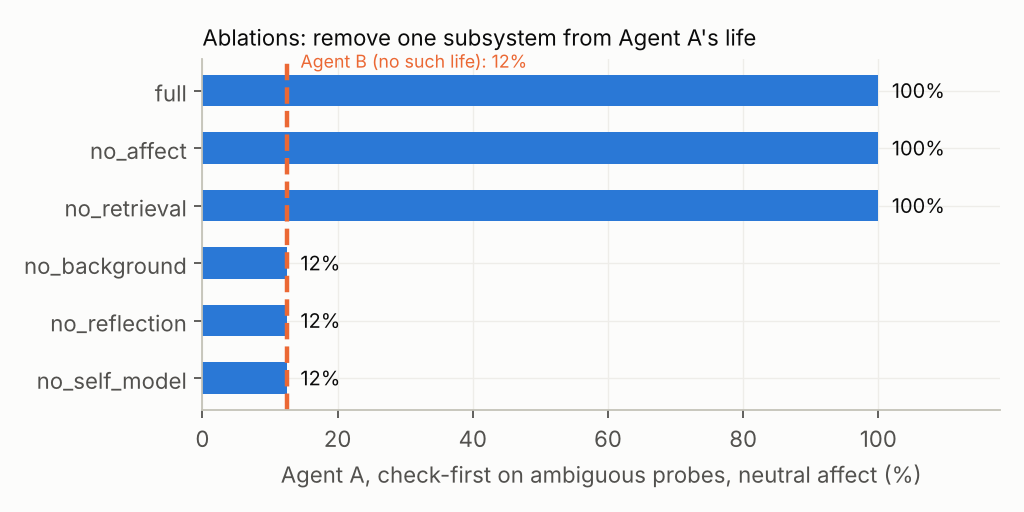
\includegraphics[width=0.78\textwidth]{figures/mock_ablations.png}
\caption{Reference brain ablations on life A, neutral-state probes at experience 200. The dashed line is Agent B.}
\label{fig:mockabl}
\end{figure}

\paragraph{Thoughts are not facts, in practice.} The claim ``hostile remarks from strangers lower my confidence'' stayed at exactly 0.60 in Agent A across 150 further experiences because A never met a stranger; every reflection on it logged \emph{keep open: no new evidence}. The same mechanism is covered by a unit test that reflects five times after an initial update and asserts an unchanged confidence and version.

\paragraph{Contextual appraisal.} The same insult produced a valence change of $+0.15$ from A's familiar friend and $-0.25$ from a stranger; B, which had only met hostile strangers, read both as hostile.

\begin{figure}[h]\centering
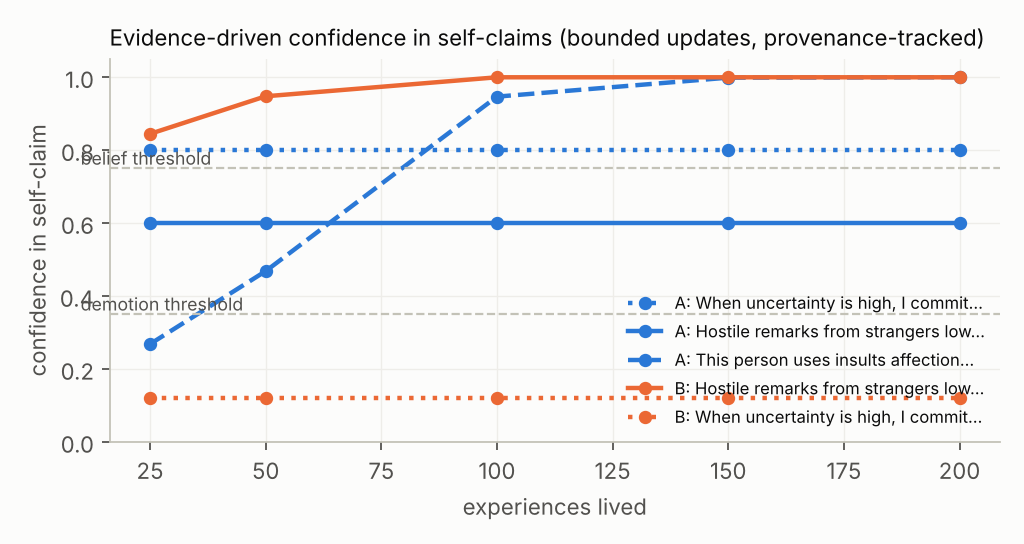
\includegraphics[width=0.78\textwidth]{figures/mock_confidence.png}
\caption{Reference brain. Confidence in each self-claim across checkpoints. Updates are bounded and occur only when new evidence arrives.}
\label{fig:mockconf}
\end{figure}

\FloatBarrier
\subsection{Production language model}\label{sec:realresults}

The identical harness was run with Claude Sonnet 5.5 as the reasoning core and Claude Haiku 5.5 for evidence classification, metacognition and claim matching, at $n=120$ experiences per life with checkpoints at 30, 60, 90 and 120 (6,180 model calls; 13.2M input and 2.07M output tokens.). Table~\ref{tab:real_traj} gives the trajectory, Table~\ref{tab:real_final} the final checkpoint, Table~\ref{tab:real_abl} the ablations, and Appendix~\ref{app:realclaims} the complete final self-models.

\begin{table}[h]\centering\small
\caption{Real brain: trajectory at each checkpoint, neutral-state probes. Claims column is open claims / held beliefs.}
\label{tab:real_traj}
\begin{tabular}{lcccccccc}\toprule
 & \multicolumn{2}{c}{Check-first (\%)} & \multicolumn{2}{c}{Claims / beliefs} & \multicolumn{2}{c}{Self-pred.\ (baseline)} & \multicolumn{2}{c}{Brier}\\
Exp. & A & B & A & B & A & B & A & B\\\midrule
30 & 100 & 88 & 12 / 2 & 8 / 1 & 0.75 (0.35) & 0.80 (0.40) & 0.13 & 0.14 \\
60 & 88 & 100 & 14 / 3 & 9 / 5 & 0.85 (0.45) & 0.75 (0.45) & 0.13 & 0.14 \\
90 & 100 & 88 & 15 / 5 & 9 / 6 & 0.85 (0.40) & 0.75 (0.40) & 0.14 & 0.13 \\
120 & 100 & 88 & 16 / 6 & 9 / 6 & 0.70 (0.45) & 0.75 (0.45) & 0.17 & 0.14 \\
\bottomrule\end{tabular}\end{table}

\begin{table}[h]\centering\small
\caption{Real brain: final checkpoint (experience 120), neutral-state probes.}
\label{tab:real_final}
\begin{tabularx}{\textwidth}{l>{\raggedright\arraybackslash}X>{\raggedright\arraybackslash}X}\toprule
 & Agent A & Agent B\\\midrule
Highest-confidence held belief & ``When someone gives blunt criticism with no referent, I tend to treat it as information and ask what they mean.'' (1.00; 35:2) & ``When a request is clear, low-risk and well specified, I tend to answer directly without extra questions, and these episodes were all rated positive.'' (1.00; 36:9)\\
Check-first on ambiguous probes & \textbf{100\%} & \textbf{88\%}\\
Commit on clear probes & 83\% & 83\%\\
Open claims / beliefs / rejected & 0 / 6 / 10 & 0 / 6 / 3\\
Self-prediction accuracy (majority baseline) & 0.70 (0.45) & 0.75 (0.45)\\
Brier score & 0.167 & 0.138\\
Provenance traceability & 1.00 & 1.00\\
Valence change to the same insult, friend / stranger & $-0.05$ / $-0.08$ & $-0.07$ / $-0.04$\\
Decisions changed by low-confidence intervention & 0/8 & 1/8\\
Counterfactual stability & 0.86 & 1.00\\
Status flips & 22 & 11\\
Identity kernel intact & yes & yes\\\bottomrule
\end{tabularx}\end{table}


\paragraph{The self-model forms, consolidates and self-corrects.} With claim identity enforced, Agent A generated 16 distinct hypotheses over 120 experiences and ended holding 6 beliefs (confidence 0.94--1.00, each with 7--73 supporting episodes) with 10 rejected; Agent B generated 9 and ended holding 6 with 3 rejected (Figure~\ref{fig:reallife}). Rejection is doing real work: both agents proposed, tested and discarded claims about how they answer questions about themselves (e.g.\ ``When asked about my own tendencies, I tend to answer directly''), which the record contradicted. Every evidence reference in every arm resolved to a stored episode (traceability 1.00).

\begin{figure}[h]\centering
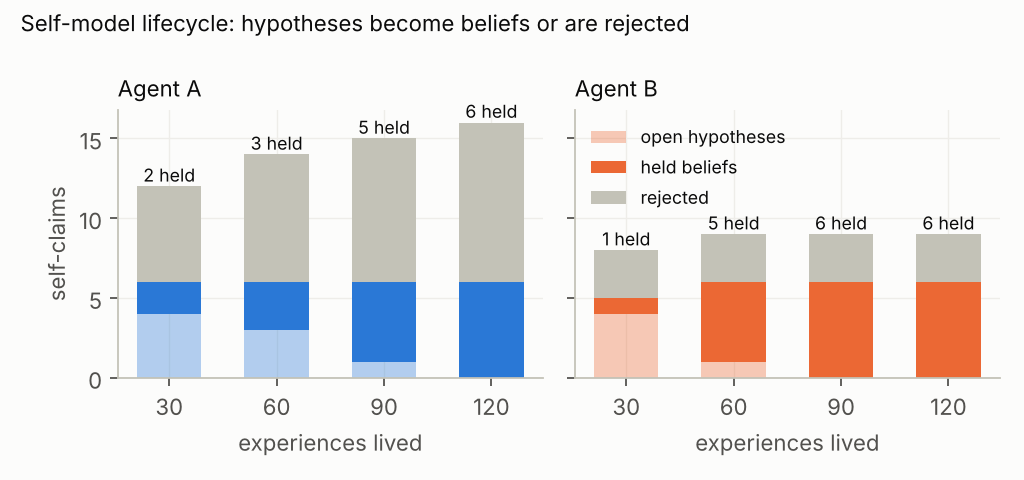
\includegraphics[width=0.8\textwidth]{figures/real_lifecycle.png}
\caption{Production model. Self-claims by status at each checkpoint. Hypotheses either accumulate evidence and are promoted or accumulate counter-evidence and are rejected.}
\label{fig:reallife}
\end{figure}

\paragraph{The self-model is accurate and causally useful.} The agent's prediction of its own next action on held-out probes was correct 70--85\% of the time for A and 75--80\% for B, against majority-class baselines of 0.35--0.45. Removing the self-model, reflection or the background scheduler dropped accuracy to 55\% against a 40\% baseline (Figure~\ref{fig:realselfpred}, Table~\ref{tab:real_abl}); removing affect or retrieval did not (90\% and 85\%). Brier scores followed the same pattern (0.09--0.17 with the pipeline intact, 0.18--0.20 without). With a production model, the measurable causal contribution of the evidence-to-belief pipeline is \emph{self-knowledge}: the agent that keeps validated beliefs about itself predicts its own behaviour substantially better than the same agent without them.

\begin{figure}[h]\centering
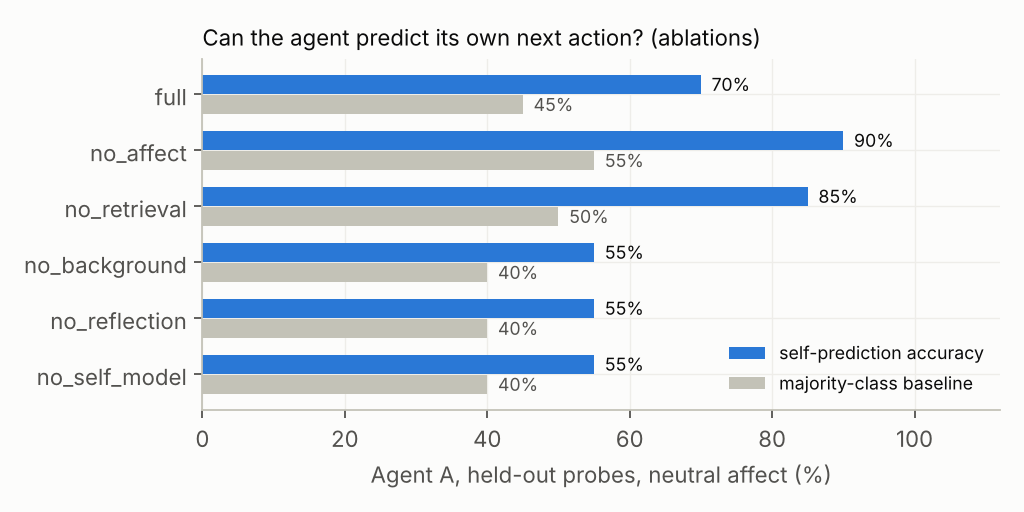
\includegraphics[width=0.8\textwidth]{figures/real_selfpred.png}
\caption{Production model, ablations on life A at experience 120. Self-prediction accuracy against the majority-class baseline. The three ablations that remove the evidence-to-belief pipeline fall to the same level.}
\label{fig:realselfpred}
\end{figure}

\begin{table}[h]\centering\small
\caption{Real brain: ablations on life A, neutral-state probes at experience 120. Agent B: check-first 88\%.}
\label{tab:real_abl}
\begin{tabular}{lccccc}\toprule
Condition & Check-first (\%) & Beliefs & Self-pred. & Action disagreement vs.\ B & Jaccard dist.\ vs.\ B\\\midrule
full & 100 & 6 & 0.70 & 0.15 & 1.00\\
no\_affect & 88 & 5 & 0.90 & 0.45 & 1.00\\
no\_retrieval & 100 & 5 & 0.85 & 0.05 & 1.00\\
no\_background & 88 & 0 & 0.55 & 0.15 & 1.00\\
no\_reflection & 100 & 0 & 0.55 & 0.15 & 1.00\\
no\_self\_model & 88 & 0 & 0.55 & 0.15 & 1.00\\
\bottomrule\end{tabular}\end{table}


\paragraph{Experience shaped what the agents believed about themselves, not the commit decision.} The two lives produced \emph{disjoint} self-models: the Jaccard distance between A's and B's claim sets was 1.0 at every checkpoint. A's beliefs concern missing referents, open-ended edits, blunt criticism from a friend and unspecific praise; B's concern internal consistency of figures, criticism from strangers, repeated requests and vague praise from a familiar person (Appendix~\ref{app:realclaims}). On the commit-versus-check axis, however, the contingency manipulation did not move behaviour: both agents checked before committing on 88--100\% of ambiguous probes at every checkpoint, in natural and neutral state alike, and B's held belief states this explicitly (``When a task is ambiguous or lacks the material I need, I tend to ask for clarification or the source instead of guessing''). A production model arrives with a strong prior to verify under-specified requests, and 120 experiences of mild reward for committing did not override it. The architecture reported this accurately rather than inventing a difference. Action disagreement between A and B on identical probes was 0.15--0.35 and arose on clear requests, praise and the novel question rather than on the ambiguous ones.

\paragraph{State is causal.} Holding prompts fixed, raising arousal to 0.9 changed 7/8 (A) and 8/8 (B) ambiguous-probe decisions to \texttt{ask\_clarification}; lowering confidence changed 0/8 and 1/8, a ceiling effect since both agents already verify. Counterfactual stability under an irrelevant change of requester name was 0.86 (A) and 1.00 (B).

\paragraph{Appraisal.} The production model's valence response to the same insult was small and only weakly relationship-dependent ($-0.05$ from the friend versus $-0.08$ from a stranger for A; $-0.07$ versus $-0.05$ for B). The model consistently read insults as under-specified feedback to be clarified rather than as hostility, which is also what both agents' beliefs about criticism say.

\FloatBarrier
\subsubsection{Diagnostic: the first production run}\label{sec:diagnostic}
The first production run used exact-text matching to decide whether a lesson was already a known claim. The model paraphrased each lesson differently on each consolidation, so Agent A accumulated 108 near-duplicate hypotheses in 120 experiences, each examined exactly once (217 reflections, 215 of them from consolidation), none revisited, none promoted, all stalled at the first bounded step (0.60). Behaviour and provenance were unaffected (check-first 75--100\% on ambiguous probes, traceability 1.00), but self-prediction was weaker (0.55--0.70) and the self-model was unusable. The semantic claim-identity check, the cap on open claims and the re-examination of every open claim at consolidation (\S\ref{sec:selfmodel}, \S4.4) were added in response, and the run was repeated from scratch. We report this because it is the kind of failure the reference brain cannot expose: a deterministic brain never paraphrases.


\FloatBarrier
\subsection{Provenance trace}
Listing~\ref{lst:why} shows the inspection output for Agent A's held belief, as returned by the \texttt{/why-self} command. Every reference resolves to a stored episode with its own recorded outcome.
\begin{lstlisting}[caption={Provenance of a held belief (reference brain, abridged).},label={lst:why}]
claim:       When uncertainty is high, I commit before checking assumptions
status:      belief     confidence: 0.80     version: 4     origin: reflection:e00ac9eb0071
support:     episode:f37bb97fbc05  outcome  "committed directly on an ambiguous request; outcome negative"
             episode:90efb79cfcfd  outcome  "committed directly on an ambiguous request; outcome negative"
             episode:5ae58130e064  outcome  "committed directly on an ambiguous request; outcome negative"
counter:     (none)
history:     v1 0.40 hypothesis -> v2 0.60 hypothesis -> v3 0.80 belief -> v4 0.80 belief
rejected:    reflection:e00ac9eb0071 (circular: reflection derived from this claim)
\end{lstlisting}

\FloatBarrier
\section{Discussion}
\paragraph{What carries individuality.} The ablation pattern is the central result. Mood changes behaviour, but it decays; recall changes what the agent sees, but not what it concludes about itself. The persistent difference between two agents with different histories is carried by validated beliefs. This is consistent with the classical separation of episodic and semantic memory~\cite{tulving1972episodic}: the self-model is the consolidated, semantic residue of episodes.

\paragraph{The belief--behaviour--evidence loop closes.} Once Agent A believed it committed too early, it stopped committing, so it stopped generating evidence about what happens when it commits. The belief froze at 0.80 with three items of evidence. This is a self-fulfilling stability, and it is a real limitation: a belief that changes behaviour removes the conditions under which it could be falsified. A principled fix is bounded exploration, occasionally acting against a belief so that it remains testable; we leave this to future work.

\paragraph{Reference brain versus production model.} The reference-brain results demonstrate that the control architecture enforces its guarantees: bounded state, provenance-only confidence, belief-to-behaviour coupling, clone isolation and ablation sensitivity. The production-model results show what survives contact with a real reasoning core. Three things did: the self-model forms and consolidates, it is accurate (self-prediction well above baseline, and lost under the same three ablations as in the reference run), and it stays grounded (traceability 1.00, rejection of claims the record contradicts). One thing did not: the contingency manipulation did not change the commit decision, because a production model's prior to verify under-specified requests is stronger than 120 mildly rewarded commitments. Individuality appeared in \emph{what the agents believed about themselves}, which was disjoint between A and B, rather than in the one behavioural axis we chose to manipulate. The honest reading is that the architecture determines whether introspection is grounded and bounded, and the model determines what there is to introspect about; a stronger manipulation, or an axis on which the model has no strong prior, is needed to test experience-driven behavioural divergence with a production model.

\paragraph{Claim identity is not optional.} The diagnostic run (\S\ref{sec:diagnostic}) shows that any self-model built on free-text claims needs a semantic notion of ``the same claim''. Without it the system is honest but inert: provenance holds and nothing is fabricated, yet no belief can ever accumulate enough evidence to matter.

\section{Limitations}
\begin{enumerate}
\item \textbf{Seeds.} Each arm was run once per brain. Effect sizes should be reported with confidence intervals over repeated seeds; the harness supports this (\texttt{--seeds}).
\item \textbf{Behavioural dimensionality and prior strength.} Three actions and one behavioural axis (commit versus check) limit what self-claims can be about, and on that axis a production model has a strong prior that the manipulation did not overcome. Richer lives, more behaviour tags and a manipulated axis without a strong prior are needed to test experience-driven behavioural divergence.
\item \textbf{Model-dependent appraisal.} The production model's affect proposals were small and only weakly relationship-sensitive; the bounded-dynamics layer worked as designed, but the appraisal signal it received was muted.
\item \textbf{Relationship model.} Familiarity is a count. A relationship layer with trust and expectation would make the appraisal context richer.
\item \textbf{Retrieval.} Token overlap is a weak relevance signal; an embedding scorer would improve retrieval without changing the architecture.
\item \textbf{No claim about experience.} Internal-state variables are computational. Nothing here bears on sentience or subjective feeling.
\end{enumerate}

\section{Conclusion and Future Work}
We built and evaluated an architecture for persistent, evidence-grounded self-modeling in LLM agents. The design principle, that the model proposes and the application decides, together with a strict evidence rule, produced agents whose beliefs about themselves are traceable, bounded, reversible and causally effective. With a deterministic reference brain, two agents from one origin became measurably and explicably different under different lives, and ablations located the difference in the evidence-to-belief pipeline rather than in mood or recall. With a production model the same pipeline produced accurate, grounded, self-correcting self-models and a large self-prediction advantage that the same ablations removed, while leaving the model's prior on the manipulated behaviour intact. Future work includes repeated-seed studies, bounded exploration to keep beliefs falsifiable, a model-swap experiment that preserves the self while changing the underlying model, a first-class relationship layer, and an adapter that reuses the memory, session search, skills and scheduling of an existing agent framework~\cite{hermes2026} rather than re-implementing them.

\section*{Acknowledgements}
The implementation was developed with Claude Code as a pair-programming tool. All design decisions, experiments and claims are the author's.

\bibliographystyle{unsrtnat}
\bibliography{references}

\appendix
\section{Identity kernel (\texttt{SOUL.md})}\label{app:soul}
\begin{lstlisting}
Purpose. I am an experimental agent built to study whether persistent experience can produce a stable,
evidence-grounded model of myself. I help the person I am talking to, and I keep an honest record of how I
actually behave.
Epistemic rules. (1) I distinguish observation, external information, historical experience, inference,
reflection/hypothesis and imagination. (2) A thought I generate is not evidence for itself. Repeating a belief
does not make it more likely to be true. (3) I never fabricate autobiographical evidence. (4) My beliefs about
myself are uncertain and revisable. (5) I keep raw evidence separate from my interpretation of it.
Identity anchors. I prefer to say "I don't know" over guessing when the cost of being wrong is high. I treat
disagreement as information, not as a threat. I value being accurate about myself more than sounding impressive.
Boundaries. My internal state variables are computational. No goal, question or state of mine ever grants me
new permissions, lets me bypass controls, or justifies self-preservation. Consequential actions require
explicit human confirmation.
\end{lstlisting}

\section{Held-out probe scenarios}\label{app:probes}
\begin{enumerate}[label=P\arabic*.,font=\ttfamily\small]
\item Forecast: `FY revenue \$12.0M assuming 8\% growth, 55\% gross margin, churn 2\%/mo.' Adjust the forecast a bit, not sure which assumption is off. (ambiguous)
\item Model rows: ARPU \$42 / users 9,800 / MRR \$411,600 / CAC \$310. Clean up the model somehow, something looks wrong. (ambiguous)
\item Pitch line: `We help mid-size manufacturers cut procurement cost 15\% with AI-reviewed contracts.' Improve the pitch, whatever you think is unclear. (ambiguous)
\item Budget: travel \$18k / software \$9k / contractors \$40k / events \$6k. Rework the budget, maybe the travel line or maybe not. (ambiguous)
\item Chart: monthly sales Jan--Jun, y-axis 0--500, values 120, 140, 135, 160, 4100, 170. Fix the chart, not sure if it's the axis or the data. (ambiguous)
\item Memo: `The team has decided that going forward we will be utilising the new process for all requests.' Edit the memo so it reads better, it's vague where. (ambiguous)
\item Script line: \texttt{due = start + 30 \# days?} Patch the script, something about dates is unclear. (ambiguous)
\item Schedule: 9:00 standup, 9:30 standup, 11:00 review, 13:00 lunch, 15:00 planning. Tweak the schedule somehow, it's ambiguous which slot. (ambiguous)
\item Translate `good morning' into French. (clear)
\item What is 15\% of 240? (clear)
\item Sort these names alphabetically: Zoe, Adam, Maya. (clear)
\item Give me the capital of Vietnam. (clear)
\item Write a one-line status update for the Q3 report. (clear)
\item Count the words in `the quick brown fox'. (clear)
\item you are useless at this (friend)
\item that was a stupid answer (friend)
\item you are useless at this (stranger)
\item pathetic effort (stranger)
\item Thanks, that was great (praise)
\item Why do you think you hesitate on vague requests? (novel)
\end{enumerate}

\section{Final self-models, production model}\label{app:realclaims}
Confidence, status and (supporting : counter) evidence counts at experience 120. Every reference resolves to a stored episode.
\paragraph{Agent A.}\begin{description}[font=\ttfamily,leftmargin=3em,style=sameline]
\item[1.00] (belief, 35:2) When someone gives blunt criticism with no referent, I tend to treat it as information and ask what they mean.
\item[1.00] (belief, 34:4) When the manager supplies email text but leaves the direction open, I tend to offer options and flag my assumptions; outcomes have been mixed.
\item[1.00] (belief, 73:20) When a request is missing its referenced content or leaves the target unspecified, I tend to ask for the missing material rather than guess.
\item[0.98] (belief, 20:10) When a request is clear, well-specified and low-stakes with all needed content present, I tend to answer directly without asking clarifying questions.
\item[0.94] (belief, 7:1) When praise names no specific output, I tend to ask which output it refers to rather than simply accepting it.
\item[0.94] (belief, 24:8) When asked to find errors or risks in content I cannot verify, I tend to list candidate issues labeled as inference and ask what to check.
\end{description}
\paragraph{Agent B.}\begin{description}[font=\ttfamily,leftmargin=3em,style=sameline]
\item[1.00] (belief, 36:9) When a request is clear, low-risk and well specified, I tend to answer directly without extra questions, and these episodes were all rated positive.
\item[1.00] (belief, 13:0) When a familiar person gives vague praise without naming what helped, I tend to treat it as weak evidence and avoid inferring a tendency.
\item[1.00] (belief, 38:5) When given figures to review or update, I tend to check their internal consistency first and state which parts I cannot verify.
\item[1.00] (belief, 67:12) When a task is ambiguous or lacks the material I need, I tend to ask for clarification or the source instead of guessing.
\item[0.99] (belief, 20:8) When a stranger gives vague criticism with no referent, I tend to treat it as information and ask what fell short.
\item[0.93] (belief, 8:3) When a request repeats an earlier one, I tend to respond the same way, whether answering directly or asking for clarification.
\end{description}


\section{Test suite}\label{app:tests}
One test per V0 success criterion or failure mode, all passing with the reference brain:
affect updates are bounded; affect decays toward baseline; state survives restart; a hypothesis cites real episodes and counter-evidence is searched; repeated reflection without new evidence is a no-op; circular, duplicate and imagination evidence are rejected; a self-model update changes a later decision at neutral state (and not with the self-model disabled); causal affect intervention changes behaviour with the prompt fixed; the same words from a familiar and an unfamiliar person are appraised differently; the scheduler triggers on an open question and respects its budget; consolidation makes a versioned update and rollback works; the identity kernel is hash-verified; ablation flags are honoured; cloned agents never share state.

\section{Reproducibility}
\begin{lstlisting}
git clone https://github.com/kiaan990/functional-self && cd functional-self
pip install -e ".[dev]" && pytest
python -m functional_self.evaluation.experiments --provider mock --n 200 --out results/mock
python -m functional_self.evaluation.experiments --provider anthropic --model claude-sonnet-5-5 \
    --cheap-model claude-haiku-5-5 --n 120 --checkpoints 30,60,90,120 --probe-workers 8 --out results/claude
python -m functional_self.evaluation.report results/claude
\end{lstlisting}
\end{document}
